\chapter{Search Algorihtms}{\label{ch:binary_search}}

Binary Search is search algorithm that reduces the normal O(n) complexiy of search to logarithmic log(n).

To binary search we need to sort our input first. There are different sorting algorithm, a few of which are listed below.
\begin{compactenum}
     \item bubble sort
     \item selection sort
     \item insertion sort
    
    \item merge sort | Based on Divide and Conquere
    \item quick sort | Based on Divide and Conquere
    \item heap sort
    \item 
    \item Radix sort
    \item \dots
\end{compactenum}

\section{Bubble Sort}
Simplest sorting algorithm.
It simulates bubbling of element to top layer, where all sorted element are present!
\begin{marginfigure}
     
\caption{Can you reason why this is not a bubble sort?}
     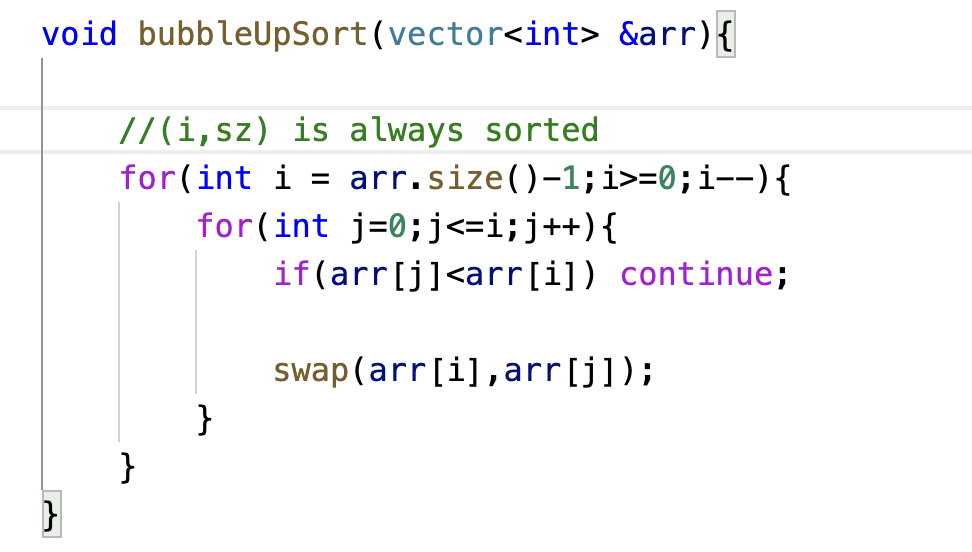
\includegraphics[width=\marginparwidth]{resources/sorting-not-bubble-sort.png}
 \end{marginfigure}

 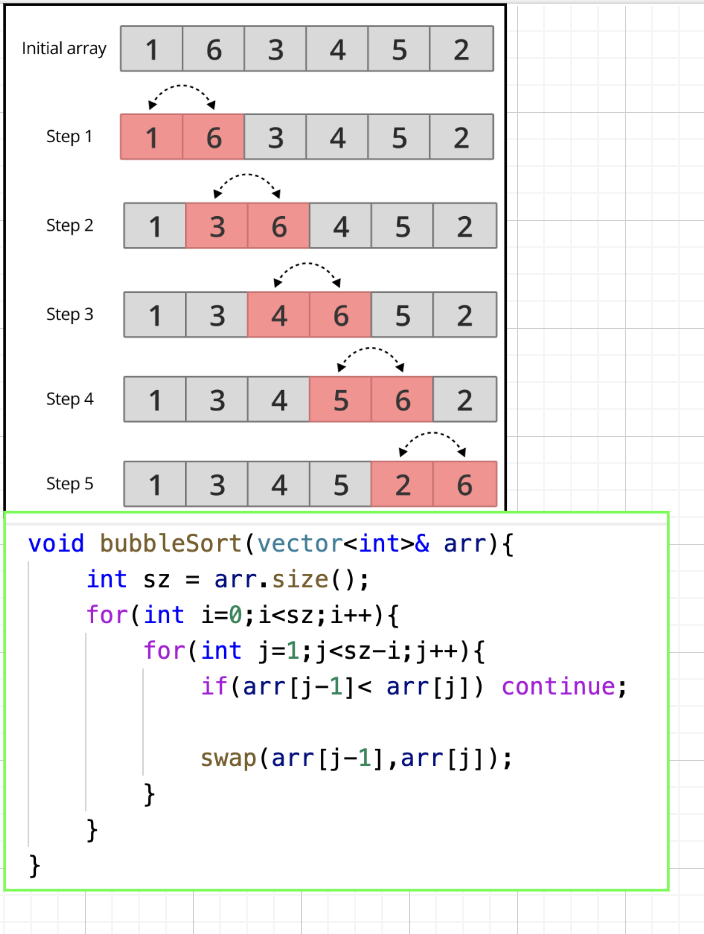
\includegraphics[width=7cm]{resources/sorting-bubble-sort.png}

 \section{Insertion Sort}
 Like we swap cards in our hands.

 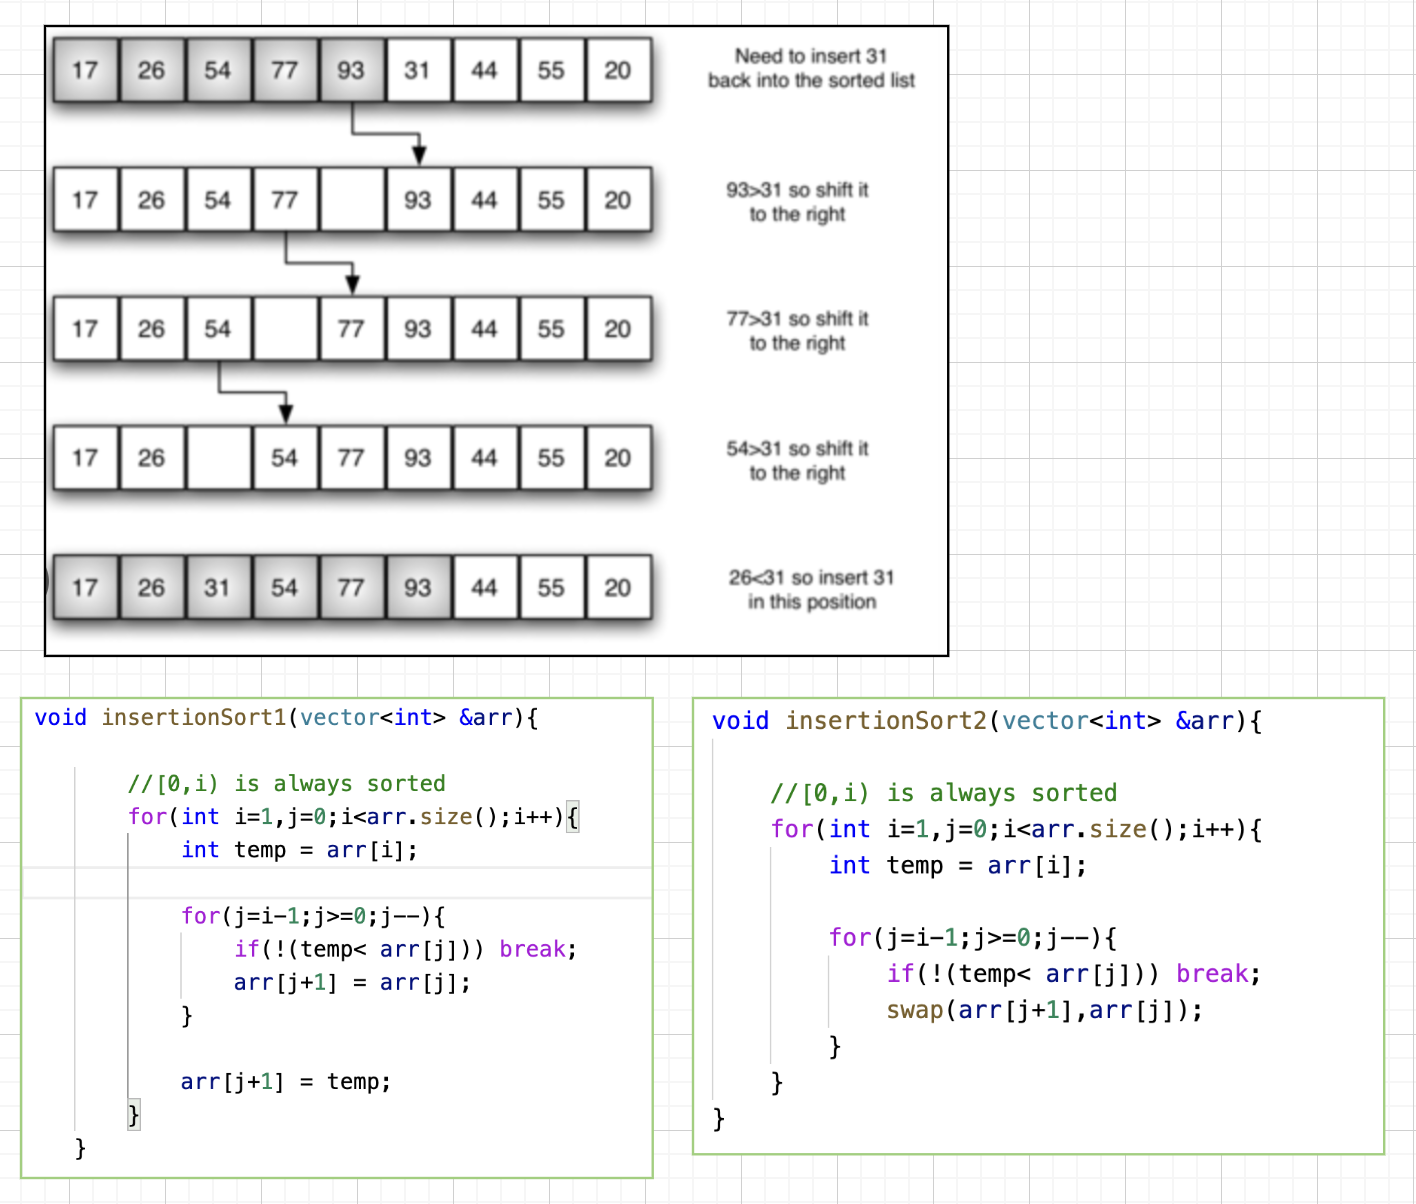
\includegraphics[width=12cm]{resources/sorting-insertion-sort.png}
 

 \section{Selection Sort}
 Select the first largest and place it on top!
 
 Select the largest element from unsorted part and then place it on the top of unsorted part!

 A Pratial example is sorting cloths on the bed! You pick biggest one, place it on box, then pick 2nd biggest one, and so on.
 
 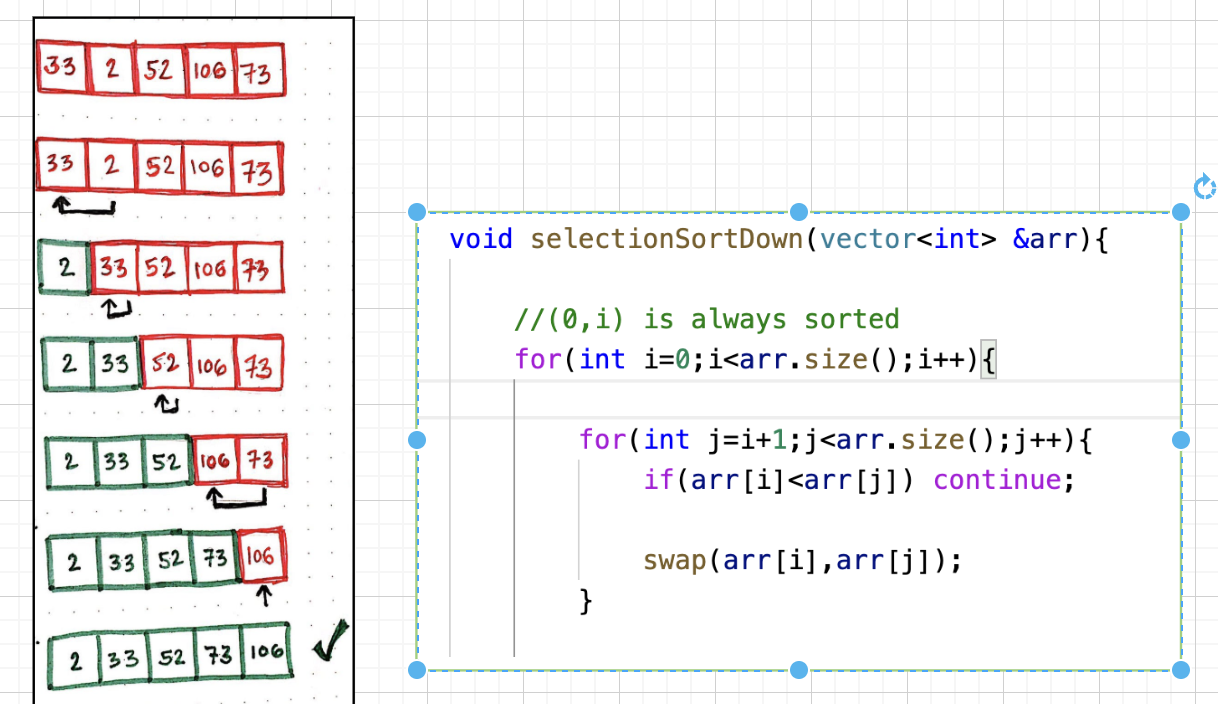
\includegraphics[width=12cm]{resources/sorting-selection-sort.png}

 \section{Merge Sort}
 Merge Sort is in-place,stable sorting algorithm. It is fastest algorith, which sort the array in $O(n*log(n))$ time.


 \begin{marginfigure}
    


     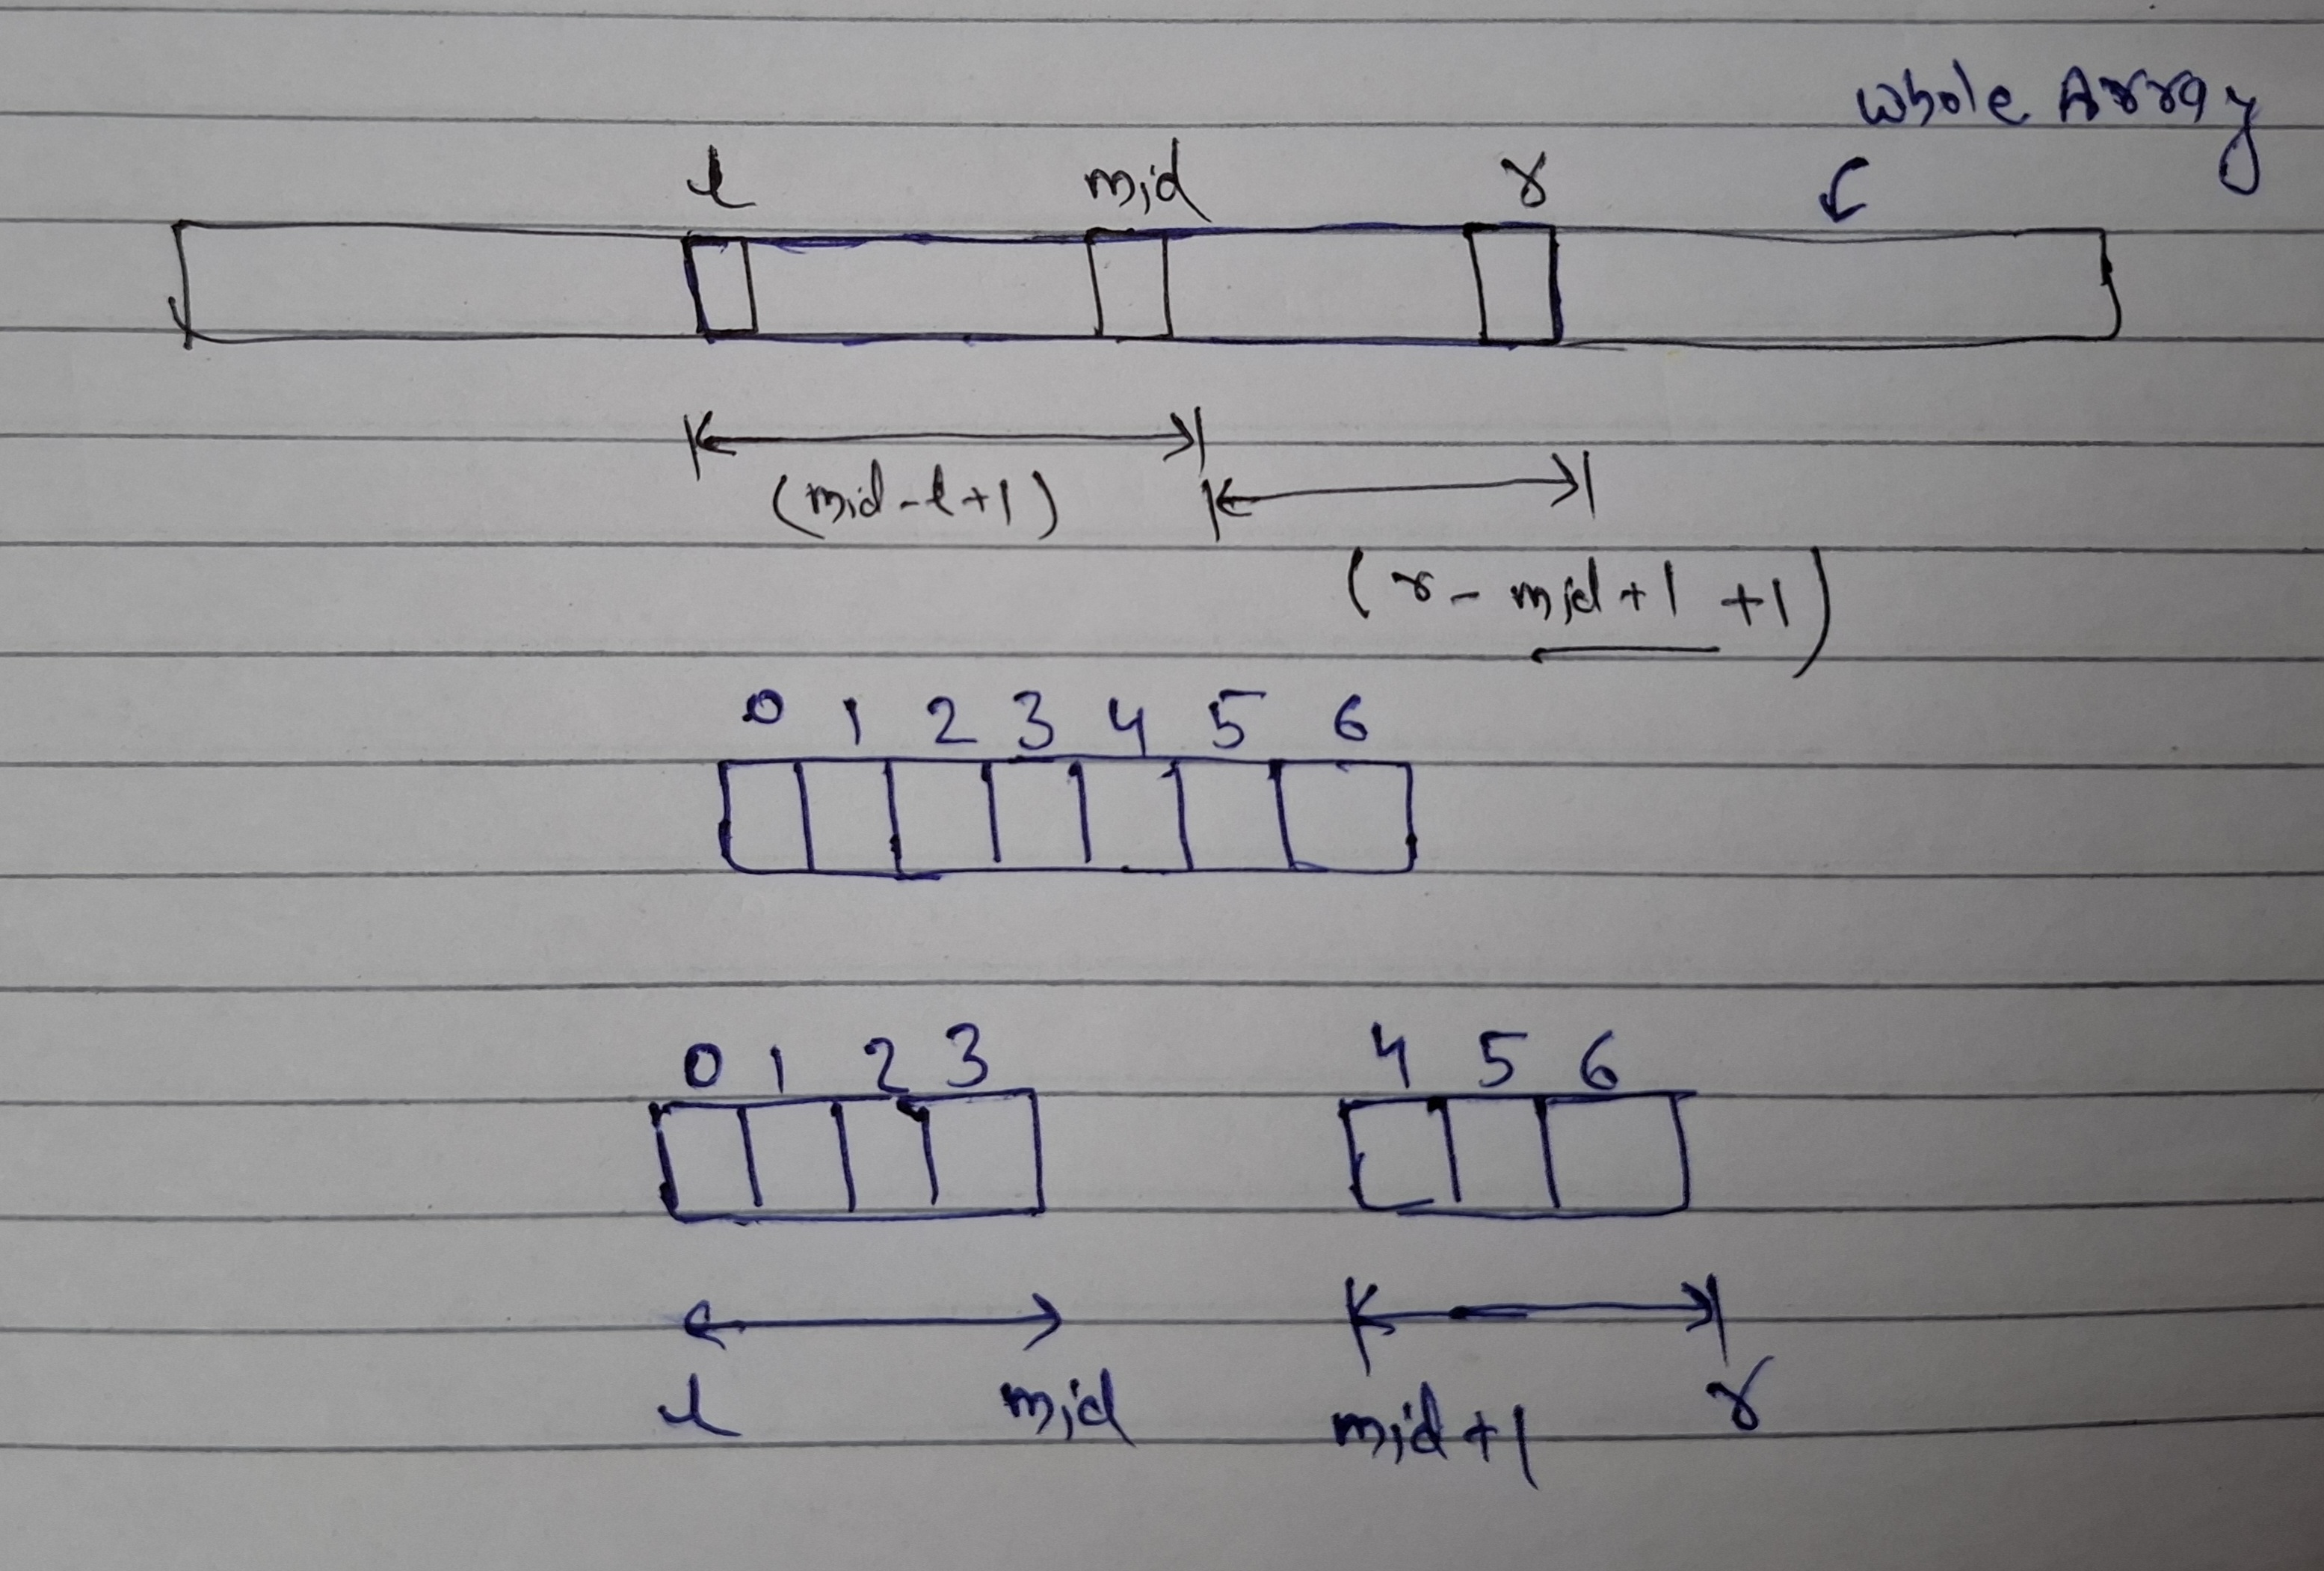
\includegraphics[width=\marginparwidth]{resources/sorting-merge-sort-division.jpg}
     \caption{visualizing array splitting in merge-sort}

 \end{marginfigure}

 \vspace{1.7cm} 
 \begin{lfigure}{resources/sorting-merge-sort-main.png}{0.6}{0.38}

     
     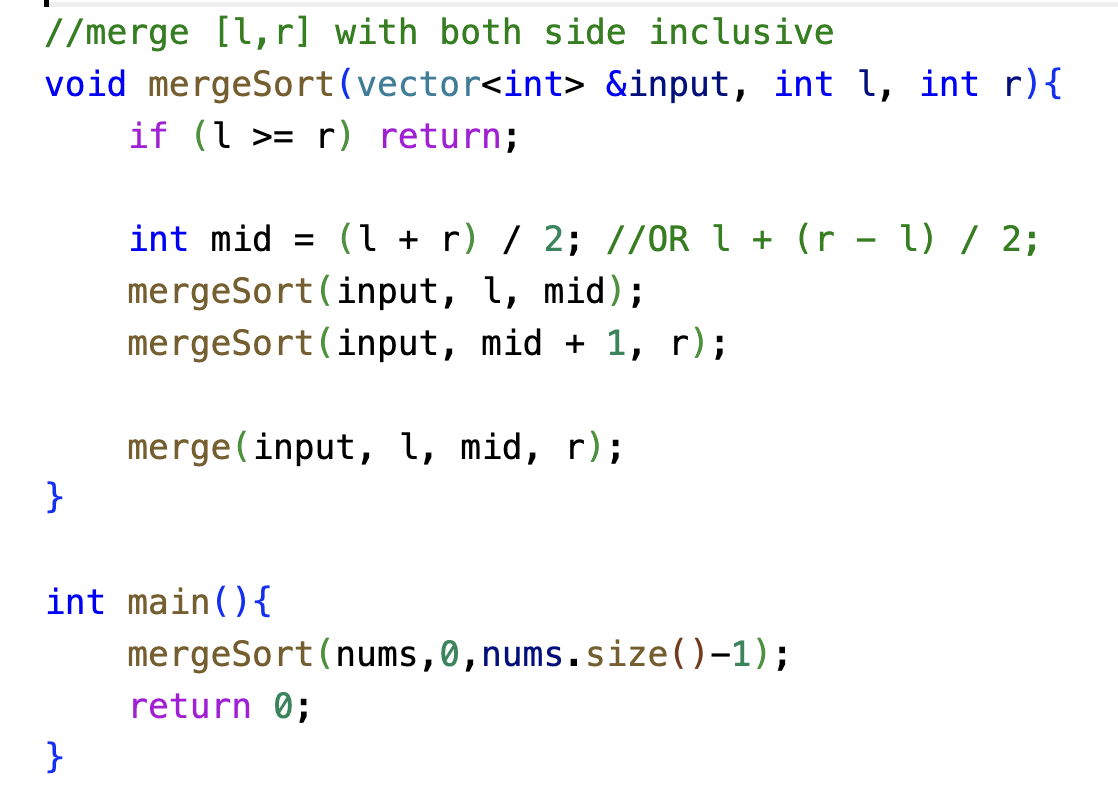
\includegraphics[width=5cm]{resources/sorting-merge-sort-base.png}

     There are 3 main part of merge sort algorithm.
     \begin{compactenum}
          \item  Split the array recursively 
          \item complete function merge(arr,l,mid,r) where [l,mid] [mid+1,r] part is sorted
          \item implement the $merge(arr,l,mid,r)$ function 
     \end{compactenum}
     \footnote{ref file: merge-sort.cpp}
 \end{lfigure}


 \section{Quick Sort}
 The quicksort algorithm has a worst-case running time of $O(n^2)$ on an input array
of n numbers. Despite this slow worst-case running time, quicksort is often the best
practical choice for sorting because it is remarkably efficient on the average: its
expected running time is  $O(nlog(n))$, and the constant factors hidden in the $O(nlog(n))$
notation are quite small. It also has the advantage of sorting in place, and it works well even in virtual-memory environments
 
$quickSort(0,arr.size()-1,arr)$
\begin{figure}
     \codecaption{Pivot Selection and Split }
     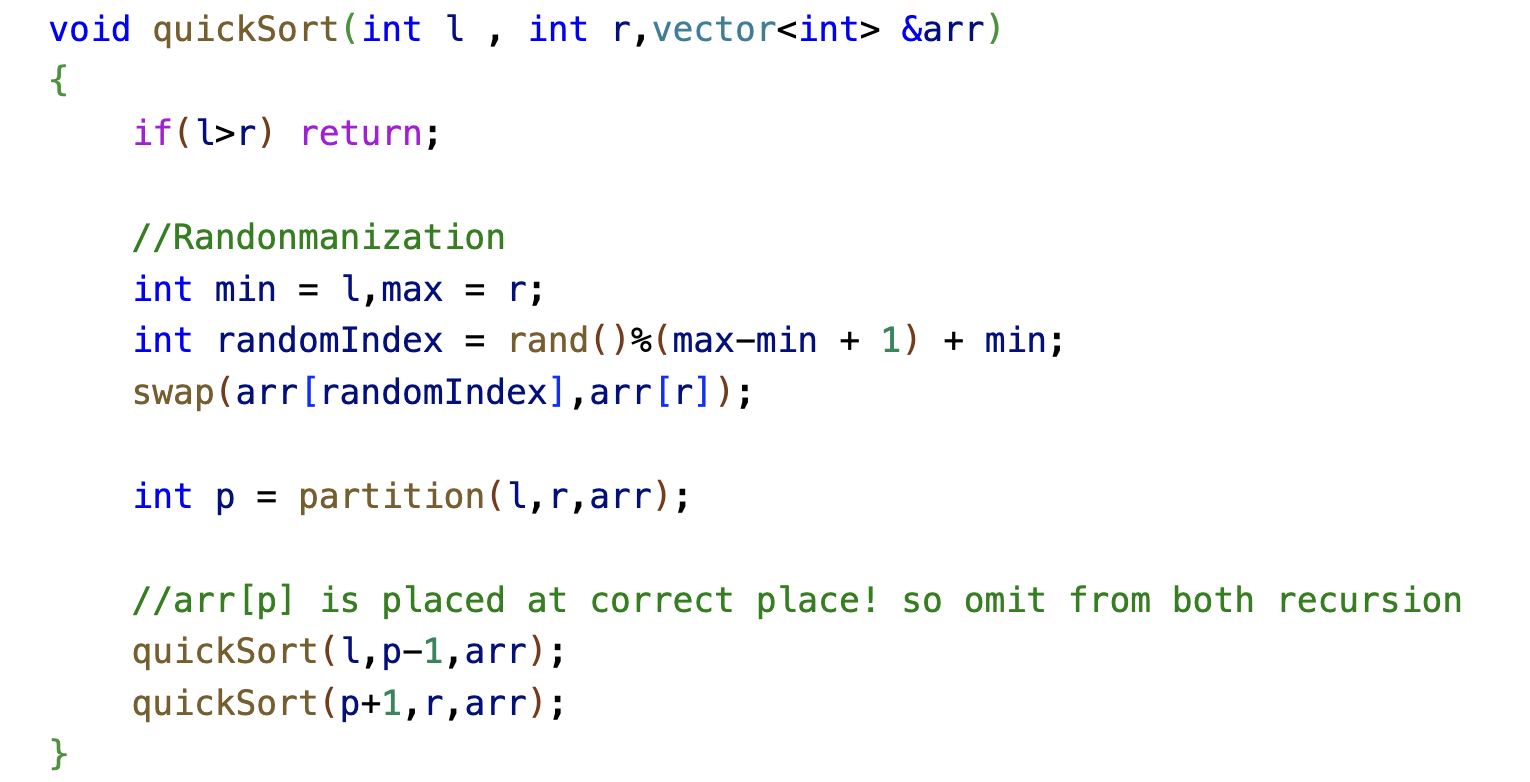
\includegraphics[width=\dimexpr\textwidth]{resources/sorting-quick-sort-1-split.png}
\end{figure}

\begin{figure}
     \codecaption{Parition Implementation}
     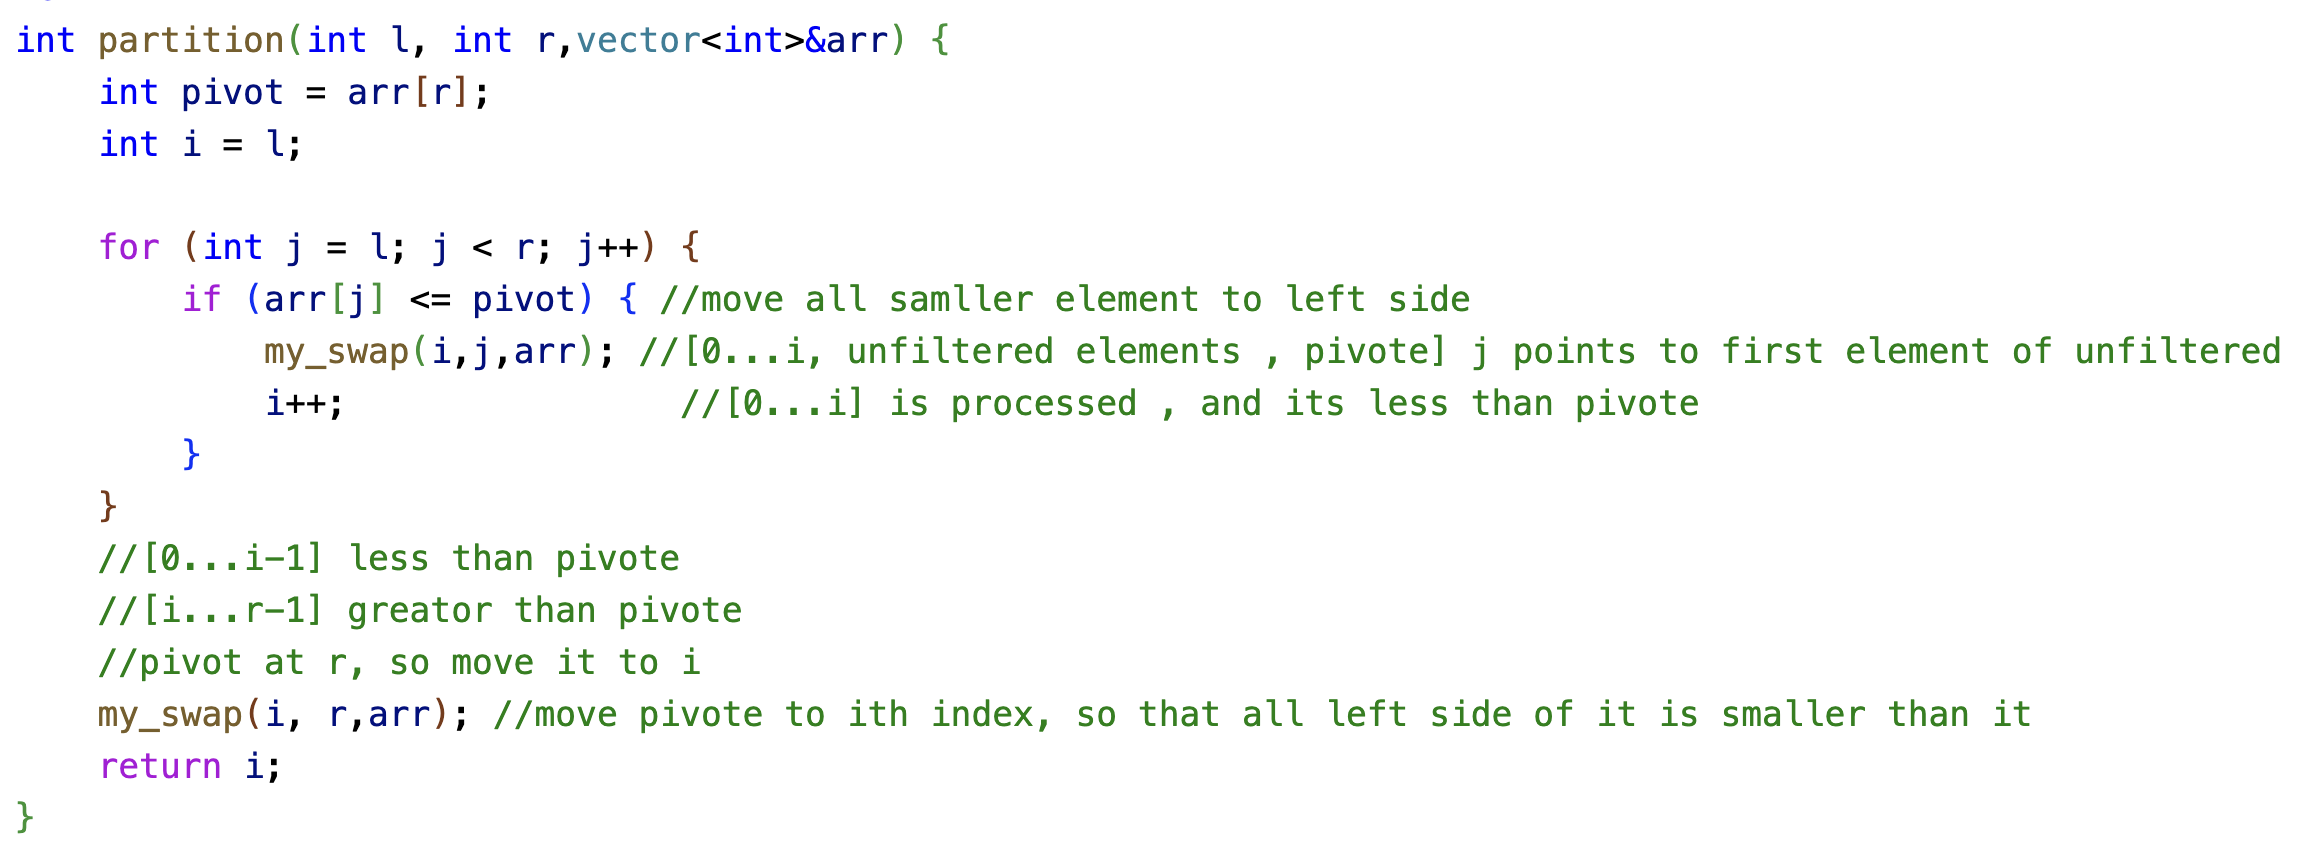
\includegraphics[width=\dimexpr\textwidth+\marginparwidth]{resources/sorting-quick-sort-2-partition.png}
\end{figure}


\begin{lfigure}{resources/sorting-quick-sort-paritition2.png}{0.45}{0.38}
     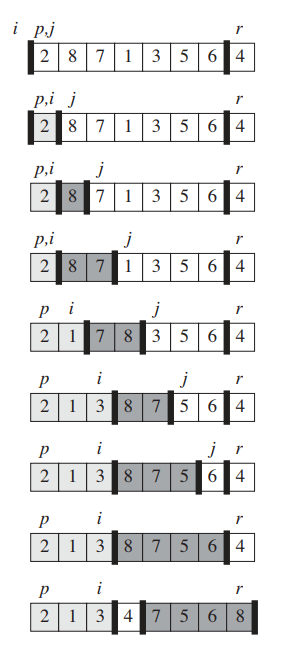
\includegraphics[width=\marginparwidth]{resources/sorting-quick-sort-paritition1.png}
\end{lfigure}

\section{Heap Sort}

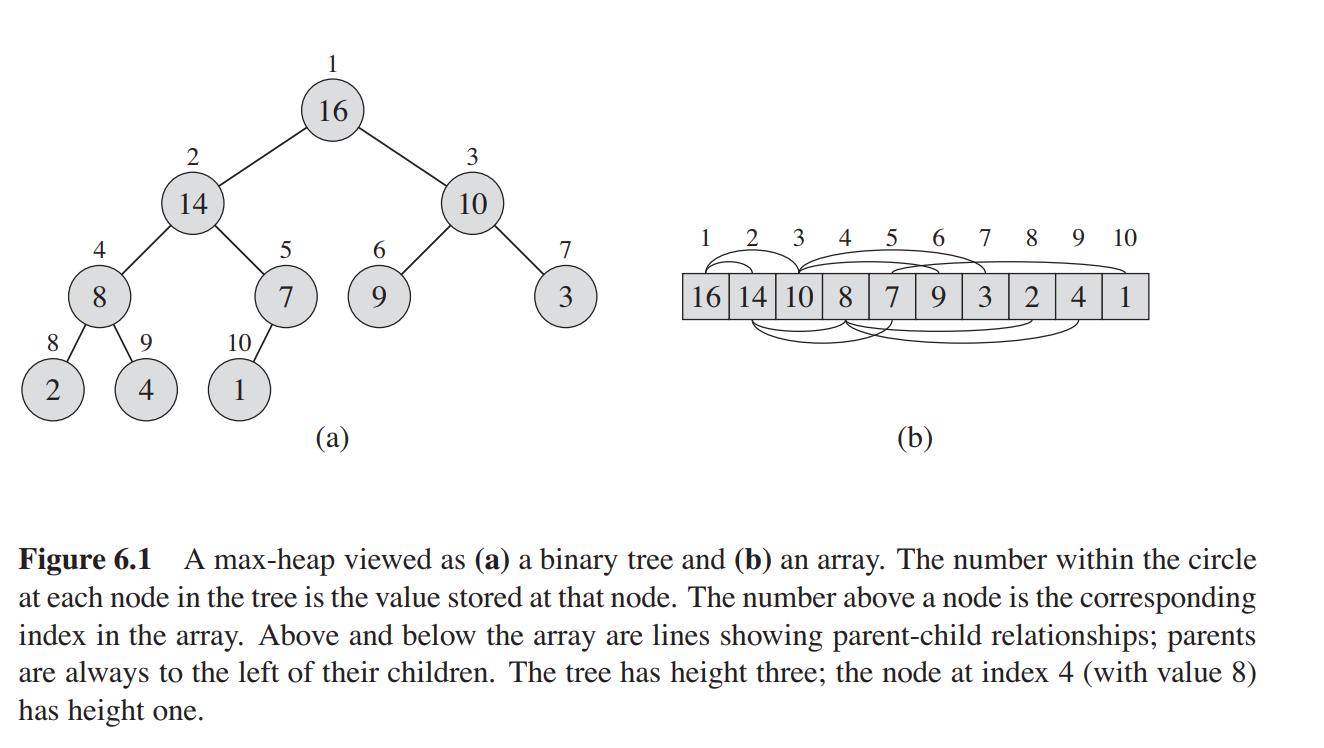
\includegraphics[width=\dimexpr\textwidth]{resources/sorting-max-heap-as-array.png}

\begin{marginfigure}
     
     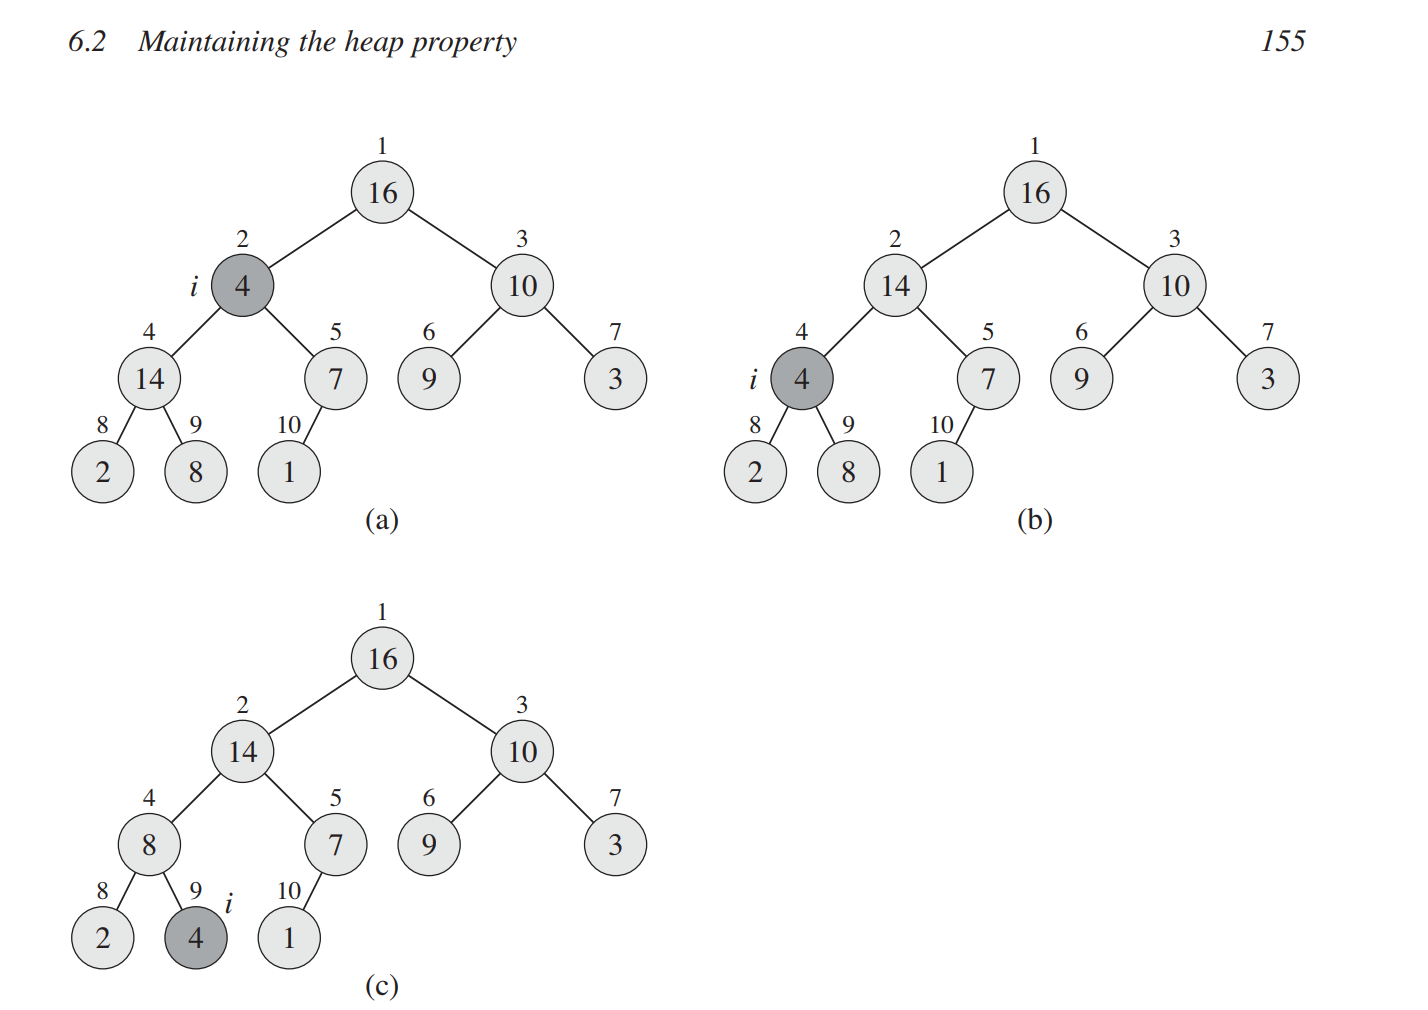
\includegraphics[width=\marginparwidth]{resources/sorting-max-heap-heapify-operation.png}
     \caption{heapify operation}
\end{marginfigure}

\begin{code3}
     class MaxHeap{
        int size;
        vector<int> harr;
         
    public:
         void heapify(int);
         void build_heap();
    
         vector<int> heapSort();
         
         void print();
         MaxHeap(vector<int> arr);          
    };
    
    vector<int> MaxHeap::heapSort(){
    
        while(size > 1){

          size--;   
          //start placing max element at end       
          swap(harr[0], harr[size-1]); 
          heapify(0);
        }

        return harr;
    }
    
    
    MaxHeap::MaxHeap(vector<int> arr):size(arr.size()){
        
        harr = vector<int>(size,-1);
    
         for(int i=0;i<size;i++)
              harr[i]=arr[i];
         
         build_heap();
    }
    
    void MaxHeap::build_heap(){
         
        /*need to heapify only non-leaf node. now let's say node k is leaf node => its left child should NOT exist => their left child will point outsie the array =>  2*k+1 > n
        => k>(n-1)/2 , Hence node for k<=(n-1)/2 all these are non-leaf nodes */
         for(int i=((size-1)/2) ; i>=0 ; i--){
              heapify(i);
         }
    }
    
    void MaxHeap::heapify(int x){
         int largest=x;
    
    /* at start, we need to find which is biggest amount these 3
                 largest
                    10
                   /  \
                 20    30
                lson   rson
    */
    
        
        if(lson < size && harr[lson] > harr[largest]) largest=lson;
        if(rson < size && harr[rson] > harr[largest]) largest=rson;
    
        if(largest == x) return; //its a perfect heap, root with x
    
        swap(harr[largest],harr[x]); 
        heapify(largest);
    }
\end{code3}
\footnote{ref: /code/heap-sort.cpp}


\section{Counting Sort}
Counting sort means, couting the frequency of element first.
Then updating the array.

Its complexiy is $O(n)$.
Its only be used when the integer range on $arr[]$ can be mapped into $<= 10^6$ unique integers.



\clearpage
\begin{exercise}[Sorting Algorithm Questions]

     \begin{compactenum}
          \item 
     \end{compactenum}

     
\end{exercise}


\begin{exercise}[Binary Search Fundamental Question List:]
    Given a sorted array write the code for following:

   \begin{compactenum}
        \item Check if element exist or not.
        \item If the element exist, return it's index else -1.
        \item If the element exist return its index,else its \verb|lower_bound|.
        \item Return \verb|lower_bound| when the array may have duplicate elements.
        \item Return \verb|upper_bound| when the array may have duplicate. How will the code change when the array do not have duplicates?
        \item use \verb|c++ stl lower_bound| to give lower bound with duplicates element.
   \end{compactenum}

   \medskip
   \begin{compactenum}      
        \item First and last occurrance of an element. (this combines all above question concept) pratice: (LC34)
        \item Find minimum element in rotate + sorted array. (LC153)
        \item (LC154) minimum in rotate+sorted when duplicate allowed.
        \item find element idx in rotate+sorted array. (LC33)
        \item find element idx in rotate+sorted array,when duplicate allowed.(LC34)
   \end{compactenum}
\end{exercise}

TO-DO: Addlower bound and upper bound image.

